\textbf{}
\section{Funktionen}
$ f:  \mathbb{D}_f \to \mathbb{W}_f \quad x \mapsto f(x) $

\subsection{Lineare Transformationen}
Eine Linear Transformation ist eine Verschiebung, Streckung oder Spiegelung der Funktions-Achsen. Dabei gilt:
\[ f := a \cdot f(bx + c) + d \]

\noindent \textbf{1:} $d$ Verschiebung nach oben/unten \\
\textbf{2:} $c$ Verschiebung bei $c>0$ nach links; $c<0$ nach rechts \\
\textbf{3:} $b$ x-Streckung; $-1$ spiegelt an der\textit{ y-Achse} \\
\textbf{4:} $a$ y-Streckung; $-1$ spiegelt an der \textit{x-Achse }\\

\subsection{Eigenschaften}
\subsubsection{Stetigkeit}
Eine Funktion heisst \textit{stetig} wenn $x \in \mathbb{D}_f$ ist und \[\lim\limits_{u^- \rightarrow x}f(u) = \lim\limits_{u^+ \rightarrow x}f(u)\]

\noindent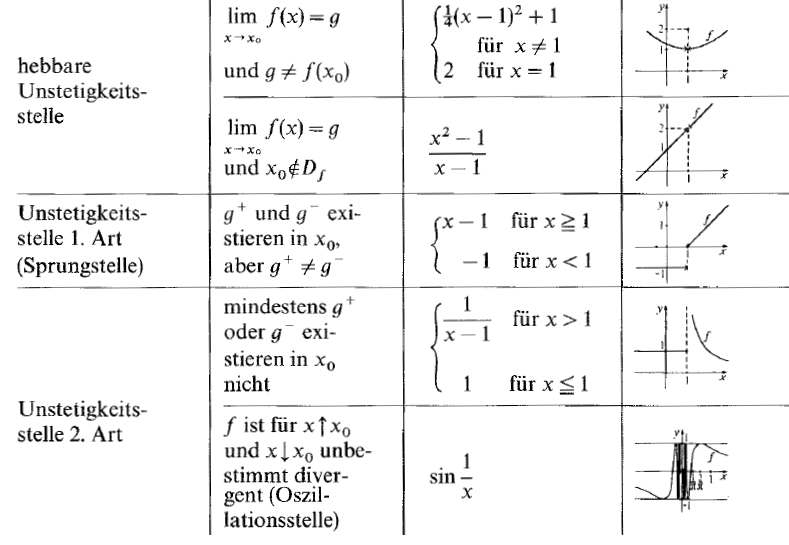
\includegraphics[width=\columnwidth]{./Images/unstetigkeit.png}

\subsubsection{Symmetrien}
\begin{tabular}{lll}
	\textbf{gerade}:& $f(-x) = f(x)$ & y-Symmetrisch\\
	\textbf{ungerade}:& $f(-x) = -f(x)$ & Nullpunkt-Symmetrisch\\
	\textbf{periodisch}:& $f(x) = f(x \pm p)$& Periode \\
\end{tabular}

\subsubsection{Monotonie}\label{monotonie}
Beschreibt das Wachstumsverhalten einer Reihe. Ungleichung muss gültig innerhalb des Intervalls $I \in [a_1;g]$ liegen ($g$: Grenzwert).\\
\noindent
\begin{tabular}{ll}
	\textbf{Wachsend $\Uparrow$ oder $\uparrow$}:& $a_{n+1} > a_n \Rightarrow a_{n+1} - a_n > 0$\\
	\textbf{Fallend $\Downarrow$ oder $\downarrow$}:& $a_{n+1} < a_n \Rightarrow a_{n+1} - a_n < 0$\\
\end{tabular}\\ \\

\noindent Die Monotonie einer Funktion kann durch die n-te Ableitung bestimmt werden.\\
\noindent\begin{tabular}{ll}
	$f \Uparrow$ & $f' > 0$\\
	$f \uparrow$ & $f' \geq 0$\\
	$f \Downarrow$ & $f' < 0$\\
	$f \downarrow$ & $f' \leq 0$\\
\end{tabular}

\subsubsection{Beschränktheit}\label{beschränkt}
Eine Funktion ist beschränkt, wenn sie ein Infimum $k$ (Grösster unterer Wert) oder Supremum $K$ (Kleinster oberer Wert) Schranke hat. Das bedeutet $k < f(x) < K$. Um $K$ herauszufinden, Reihe $a_n \lessgtr K$ und nach $n$ auflösen. Oft wird eine Abschwächen zB $a_n \eqi \frac{n^2+1}{n+1} > \frac{n^2}{n+1} > \frac{n^2}{2n} = \frac{n}{2}$ verwendet. Hinweis: Grenzwertgleichung!

\subsubsection{Umgebung}
Umgebung ($g$: Grenzwert, $a_n$ Folge, $e$ Umgebung): $\left|a_n - g\right| < \epsilon$


\subsubsection{Konvergenz / Divergenz}
Eine Funktion/Reihe ist \textbf{Konvergent}, wenn sie Beschränkt + Monoton ist. Andernfalls ist sie \textbf{Divergent}.
Konvergenz bestimmen:
\begin{enumerate}[nosep]
	\item Grenzwert berechnen (\underline{Hinweis}: Grenzwertgleichung, \verweiseref{einschliessungsprinzip}, \verweiseref{bolzano}, \verweiseref{induktion})
	\item \verweiseref{monotonie} prüfen 
	\item Beschränktheit prüfen anha0nd der Monotonie
\end{enumerate}

\subsubsection{Konvexität / Wendepunkt}
Auch als Krümmungsverhalten bekannt. (Siehe auch \bronstein{253})\\
\begin{minipage}{\textwidth}	
	\begin{minipage}{0.2\textwidth}
		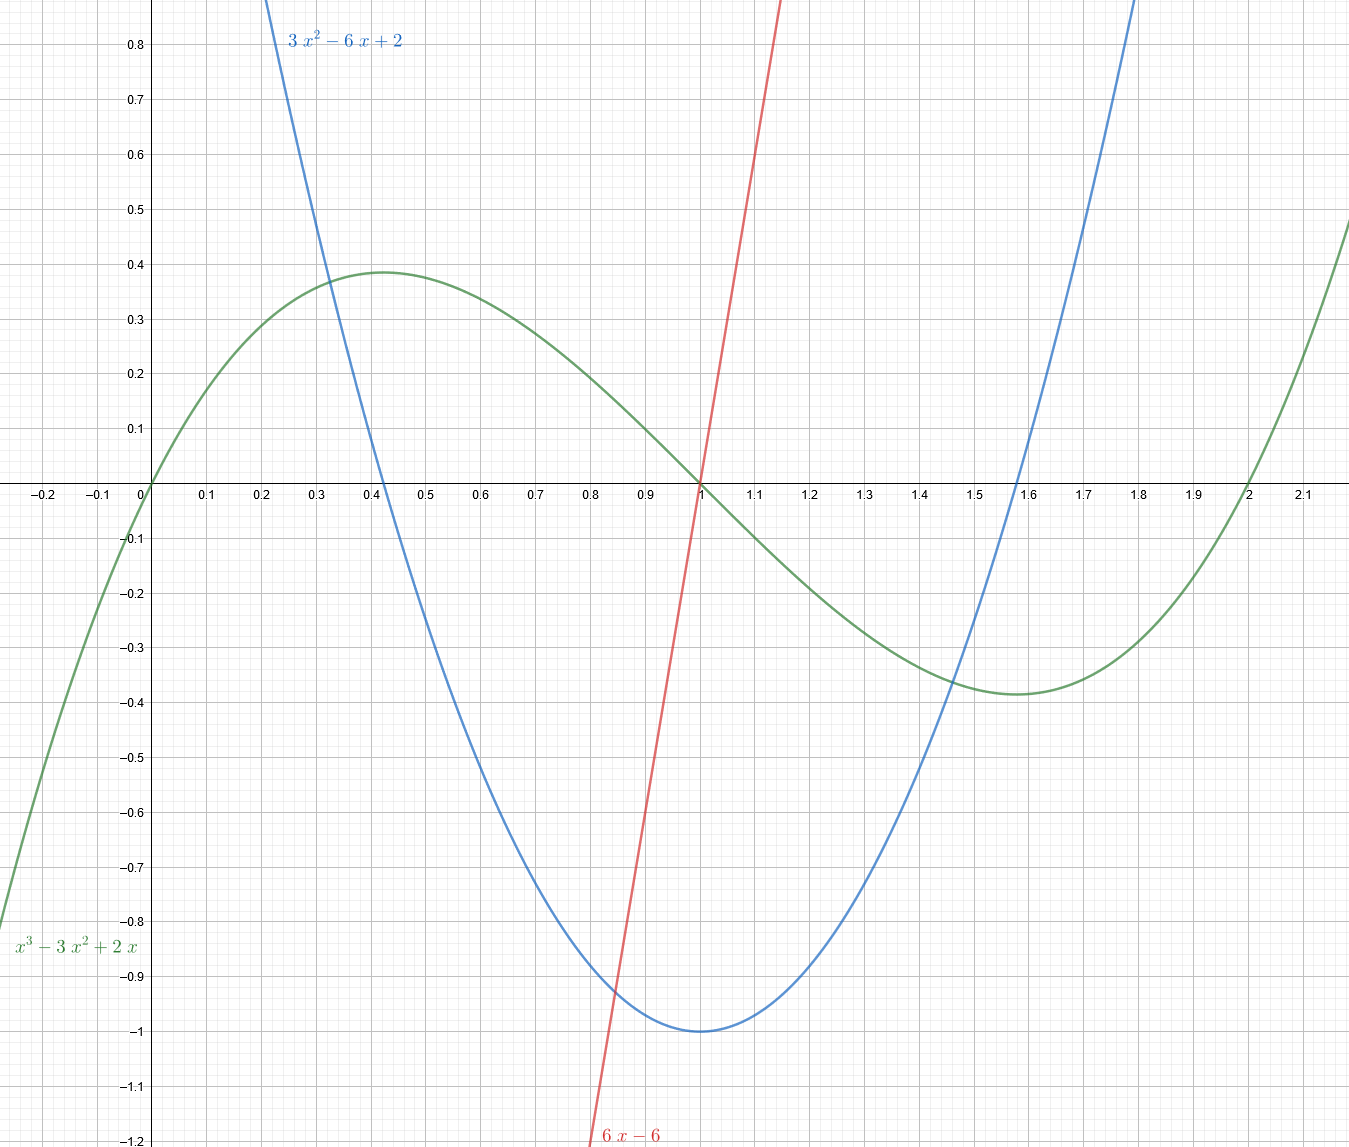
\includegraphics[width=\linewidth,keepaspectratio=true]{./Images/konvexkonkav.png}
	\end{minipage}%%% to prevent a space
	\begin{minipage}{0.3\textwidth}	
		\begin{itemize}[nosep]
			\item \textbf{Konvex} (Links Kurve):\\ $f'' > 0$ 
			\item \textbf{Streng Konvex} (Links Kurve):\\ $f'' \geq 0$ 
			
			\item \textbf{Konkav} (Rechts Kurve):\\ $f'' < 0$ 
			\item \textbf{Streng Konkav} (Rechts Kurve):\\ $f'' \leq 0$ 
			
			\item \textbf{Wendepunkt}:\\ Extremstelle 1.Ableitung, oder $f'' = 0$
		\end{itemize}
	\end{minipage}
\end{minipage}

\subsubsection{Asymptote \bronstein{259}}
Annähernde Kurve in 3 Typen (ZG: Zähler-Grad, NG: Nenner-Grad):\\
\begin{tabular}{p{1.5cm}p{3.1cm}p{4.2cm}}
	ZG $<$ NG & & $\frac{x}{x^2 - 4} \Rightarrow y = 0$ \\
	ZG $=$ NG & Quotient aus Koeffizienten von grössten Grad. & $\frac{2x-6}{x+4} \Rightarrow y = \frac{2}{1}$ \\
	ZG $>$ NG & Polynomdivision & $\frac{x^2 + 2x + 1}{x - 1} \Rightarrow \underbrace{x + 3}_{Asymptote} + \frac{4}{x -1}$
\end{tabular}

\noindent Echt-Gebrochen: ZG $<$ NG, Unecht-Gebrochen: ZG $>$ NG

\subsection{Schnittwinkel}
Schnittwinkel zwischen zwei Geraden ($m: \text{Steigung} = f'(x)$):
\[ \tan(\alpha) = \frac{m_1 - m_2}{1 + m_1m_2} \]

\noindent Für Schnittwinkel $\alpha$ an Y-Achse, $g(x) = 0$ verwenden und Winkel $\beta$ an X-Achse berechnen. Anschliessend $90-\beta = \alpha$ rechnen.\\


\subsection{Nullstellen}
\noindent abc-Formel $x_{1,2} = \frac{-b\pm\sqrt{b^2-4ac}}{2a}$

\noindent Horner-Schema \\
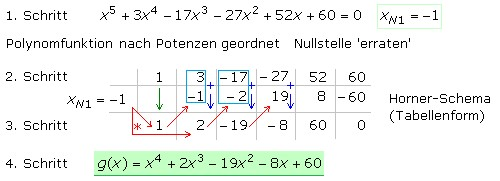
\includegraphics[width=\columnwidth]{./Images/horner.jpg}


\subsection{Partialbruchzerlegung}
Jede echt gebrochen rationale Funktion $R(x)$ kann in ein Partialbruch zerlegt werden.
\begin{enumerate}[nosep]
	\item evt. Polynom-Division
	\item Jedes Produkt als Division darstellen (mit entsprechendem Fall \bronstein{15})
	\item Auf einen HN bringen und mit original Gleichsetzen.
	\item Koeffizientenvergleich oder Nullstellen finden
\end{enumerate}

\subsection{Trigonometrisch}

$ \text{rad} = \frac{\pi}{180°} \cdot \text{deg} \quad;\quad \text{deg} = \frac{180}{\pi} \cdot \text{rad} $


\begin{table}[ht]
	\centering
	\begin{tabular}{c|c|c|c|c|c|c|c|c|c}
		\rowcolor{LightGray}
		$\alpha$  & 0 & $\frac{\pi}{6}$ & $\frac{\pi}{4}$ & $\frac{\pi}{3}$ & $\frac{\pi}{2}$ & $\frac{2\pi}{3}$ & $\frac{3\pi}{4}$ & $\frac{5\pi}{6}$ & $\pi$ \\
		\rowcolor{LightGray}
		\tiny{$\alpha$°} & \tiny{0} & \tiny{30} & \tiny{45} & \tiny{60} & \tiny{90} & \tiny{120} & \tiny{135} & \tiny{150} & \tiny{180} \\
		\Xhline{2\arrayrulewidth}

		$\sin\alpha$ & 0 & $\frac{1}{2}$ & $\frac{\sqrt{2}}{2}$ & $\frac{\sqrt{3}}{2}$ & 1 & $\frac{\sqrt{3}}{2}$ & $\frac{\sqrt{2}}{2}$ & $\frac{1}{2}$ & 0 \\
		\hline
		$\cos\alpha$ & 1 & $\frac{\sqrt{3}}{2}$ & $\frac{\sqrt{2}}{2}$ & $\frac{1}{2}$ & 0 & -$\frac{1}{2}$ & $\frac{\sqrt{2}}{2}$ & $\frac{\sqrt{3}}{2}$ & -1 \\
		\hline
		$\tan\alpha$ & 0 & $\frac{1}{\sqrt{3}}$ & 1 & $\sqrt{3}$ & / & -$\sqrt{3}$ & -1 & -$\frac{1}{\sqrt{3}}$ & 0
	\end{tabular}
	\begin{tabular}{c|c|c|c|c|c|c|c|c}
		\rowcolor{LightGray}
		$\alpha$  & $\frac{7\pi}{6}$ & $\frac{5\pi}{4}$ & $\frac{4\pi}{3}$ & $\frac{3\pi}{2}$ & $\frac{5\pi}{3}$ & $\frac{7\pi}{4}$ & $\frac{11\pi}{6}$ & $2\pi$ \\
		\rowcolor{LightGray}
		\tiny{$\alpha$°} & \tiny{210} & \tiny{225} & \tiny{240} & \tiny{270} & \tiny{300} & \tiny{315} & \tiny{330} & \tiny{360} \\
		\Xhline{2\arrayrulewidth}
		
		$\sin\alpha$ & -$\frac{1}{2}$ & -$\frac{\sqrt{2}}{2}$ & -$\frac{\sqrt{3}}{2}$ & -1 & -$\frac{\sqrt{3}}{2}$ & -$\frac{\sqrt{2}}{2}$ & -$\frac{1}{2}$ & 0 \\
		\hline
		$\cos\alpha$ & -$\frac{\sqrt{3}}{2}$ & -$\frac{\sqrt{2}}{2}$ & -$\frac{1}{2}$ & 0 & $\frac{1}{2}$ & $\frac{\sqrt{2}}{2}$ & $\frac{\sqrt{3}}{2}$ & 1  \\
		\hline
		$\tan\alpha$ & $\frac{1}{\sqrt{3}}$ & 1 & $\sqrt{3}$ & / & -$\sqrt{3}$ & -1 & -$\frac{1}{\sqrt{3}}$ & 0
	\end{tabular}
\end{table}

\noindent Beziehungen:\\
\begin{tabular}{>{\(}l<{\)} @{\(\;=\;\)} >{\(}r<{\)}   >{\(}l<{\)} @{\(\;=\;\)} >{\(}r<{\)} }
	\cos(\alpha + 2\pi) & \cos(\alpha) & \sin(\alpha + 2\pi) & \sin(\alpha) \\
	\cos(-\alpha)                & \cos(\alpha)  & \sin(-\alpha)                & -\sin(\alpha) \\
	\cos(\pi - \alpha)           & -\cos(\alpha) & \sin(\pi - \alpha)           & \sin(\alpha)  \\
	\cos(\frac{\pi}{2} - \alpha) & \sin(\alpha)  & \sin(\frac{\pi}{2} - \alpha) & \cos(\alpha) \\
	\midrule
\end{tabular}
\begin{align*}
	1 &= \cos^2(\alpha) + \sin^2(\alpha) \\
	\midrule
	\sin(\alpha \pm \beta) &= \sin(\alpha)\cos(\beta) \pm \cos(\alpha)\sin(\beta) \\
	\cos(\alpha \pm \beta) &= \cos(\alpha)\cos(\beta) \mp \sin(\alpha)\sin(\beta) \\
	\tan\alpha \pm \beta &= \frac{\tan(\alpha)\cdot\tan(\beta)}{1\mp\tan(\alpha)\cdot\tan(\beta)} \\
	\midrule
	1 &= \cosh^2(\alpha) - \sinh^2(\alpha) \\
	\sinh(\alpha) &= \frac{e^\alpha - e^{-\alpha}}{2}\\
	\cosh(\alpha) &= \frac{e^\alpha + e^{-\alpha}}{2}\\
	\arcsinh(\alpha) &= \ln(\alpha + \sqrt{\alpha^2 + 1})\\
	\arccosh(\alpha) &= \ln(\alpha + \sqrt{\alpha^2 - 1})
\end{align*}


